\chapter{Análise de séries temporais}
\label{Capitulo:analisedeseriestemporais}

O objetivo deste capítulo é a introdução de alguns conceitos relativos a séries
temporais e modelos utilizados para modelá-las e prever seus próximos valores.

\section{Conceitos iniciais}

Existem, na literatura, diversas definições para o termo \emph{série temporal}.
A definição proposta em~\citep{Livro:analiseseriestemporais} parece ser mais
abrangente. Nela, o autor caracteriza uma série temporal como uma realização de
um processo estocástico. Já~\citep{Livro:estatisticaadmeeconomia} a conceitua
como dados observados em~\emph{n} períodos, restringindo sua definição a séries
temporais discretas. O mesmo faz~\citep{Livro:serietemporal2}, onde as séries
temporais são formalmente definidas como um conjunto de variáveis aleatórias
indexadas no tempo. Neste trabalho as séries temporais sempre serão discretas.
Portanto, as três definições acima são aceitáveis.

Uma série temporal pode ser caracterizada, ainda, como estacionária ou não
estacionária. Uma série estacionária é aquela que flutua ao redor de uma média
ao longo do tempo. A Figura~\ref{fig:exestacionaria} apresenta o exemplo de uma
série estacionária, enquanto na Figura~\ref{fig:exnaoestacionaria} é exibido um
exemplo de uma série não estacionária. A fim de se tornar uma série não
estacionária em estacionária, calcula-se a diferença entre seus termos
consecutivos. Seja $Z$ uma série temporal e $\Delta^d$ o operador diferença,
sendo $d$ a quantidade de diferenças a ser calculada, a
Equação~\ref{eq:diferenca} mostra a criação de uma nova série, $W$, formada pela
$d$-ésima diferença da série $Z$.

\begin{figure}[ht]
\centering
\begin{subfigure}{.49\textwidth}
  \centering
  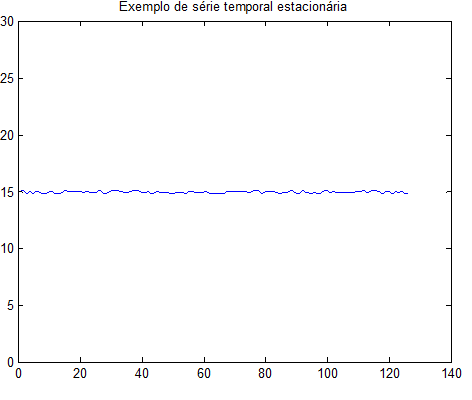
\includegraphics[width=1\linewidth]{fig/serieestacionaria.png}  
  \caption{Exemplo de série estacionária.}
  \label{fig:exestacionaria}
\end{subfigure}%
\hfill
\begin{subfigure}{.49\textwidth}
  \centering
  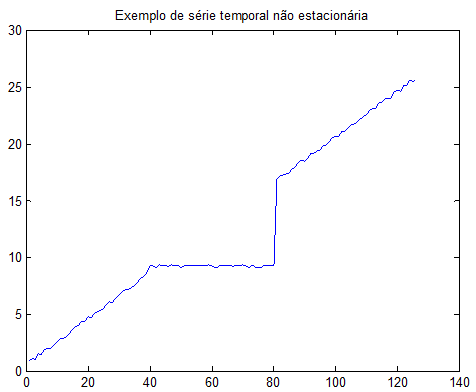
\includegraphics[width=1\linewidth]{fig/serienaoestacionaria.png}
  \caption{Exemplo de série não estacionária.}
  \label{fig:exnaoestacionaria}
\end{subfigure}
\caption{À esquerda o exemplo de uma série estacionária. À direita o exemplo de
uma série não estacionária.}
\label{fig:naoestacionariaeestacionaria}
\end{figure}

\begin{equation}
W = \Delta^dZ
\label{eq:diferenca}
\end{equation}

\begin{figure}[ht]
\centering
\begin{subfigure}{.49\textwidth}
  \centering
  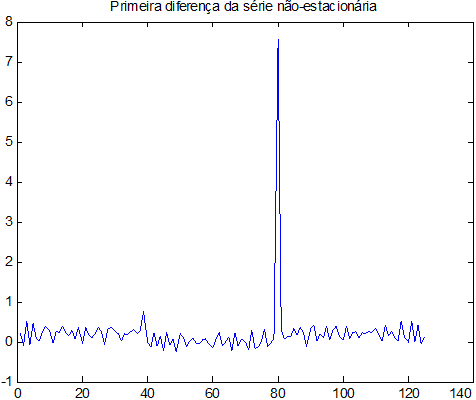
\includegraphics[width=1\linewidth]{fig/serieprimeiradiferenca.png}  
  \caption{Resultado da aplicação da equação~\ref{eq:diferenca} com $d=1$ na
  figura~\ref{fig:exnaoestacionaria}.}
  \label{fig:d1}
\end{subfigure}%
\hfill
\begin{subfigure}{.49\textwidth}
  \centering
  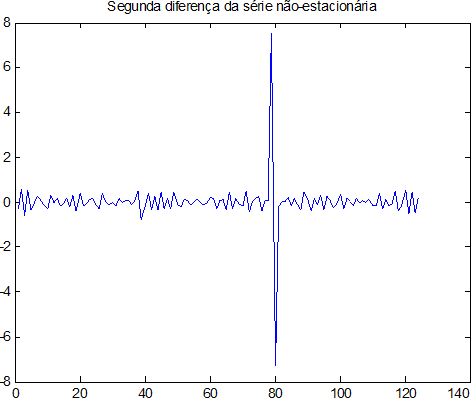
\includegraphics[width=1\linewidth]{fig/seriesegundadiferenca.png}
  \caption{Resultado da aplicação da equação~\ref{eq:diferenca} com $d=2$ na
  figura~\ref{fig:exnaoestacionaria}.}
  \label{fig:d2}
\end{subfigure}
  \caption{Tornando a figura~\ref{fig:exnaoestacionaria} em
  estacionária através da equação~\ref{eq:diferenca}.}
\label{fig:d1ed2}
\end{figure}

Aplicando-se a Equação~\ref{eq:diferenca} sobre a série da
Figura~\ref{fig:naoestacionariaeestacionaria}, obtem-se os resultados expostos
na Figura~\ref{fig:d1ed2}. É possível ver que, para $d=1$, a série ainda não se
tornou estacionária, necessitando de mais uma diferença para fazê-lo. Em geral, duas diferenças são suficientes para tornar
a série estacionária~\citep{Livro:analiseseriestemporais}.

Uma série temporal é dita~\emph{homocedástica} se sua variância puder ser
considerada constante ao longo do tempo. Caso contrário, a série é chamada
de~\emph{heteroscedástica}. A Figura~\ref{Figura:exemplodedadohomocedastico}
apresenta uma série temporal homocedástica ao passo que as
Figuras~\ref{Figura:exemplodedadoheterocedasticosismico}
e~\ref{Figura:exemplodedadoheterocedasticoaudio} apresentam exemplos de dados
heteroscedásticos.

\begin{figure}[!ht]
\centering
\begin{subfigure}{.49\textwidth}
  \centering
  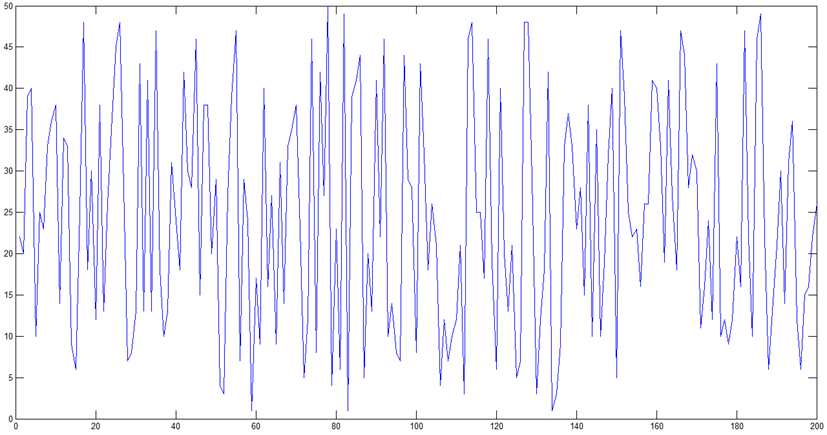
\includegraphics[width=1\linewidth]{fig/homocedastico.png}  
  \caption{Exemplo de dado homocedástico}
  \label{Figura:exemplodedadohomocedastico}
\end{subfigure}%
\hfill
\begin{subfigure}{.49\textwidth}
  \centering
  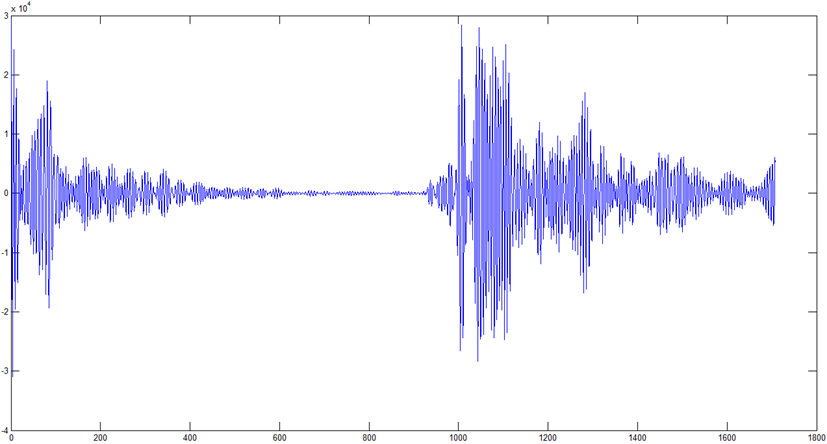
\includegraphics[width=1\linewidth]{fig/tracosismico.png}
  \caption[Exemplo de dado heteroscedástico]{O traço sísmico é um exemplo de
  dado heteroscedástico}
  \label{Figura:exemplodedadoheterocedasticosismico}
\end{subfigure}\\[1ex]
\begin{subfigure}{.49\textwidth}
  \centering
  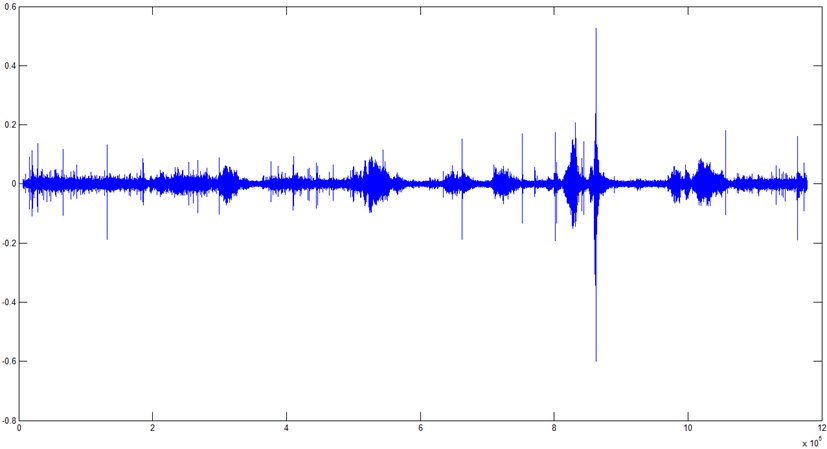
\includegraphics[width=1\linewidth]{fig/tracoaudio.png}
  \caption{O dado de áudio gerado por voz humana e captado por um microfone
  também é exemplo de dado heteroscedástico.}
  \label{Figura:exemplodedadoheterocedasticoaudio}
\end{subfigure}
  \caption{Exemplos de dados homo e heterocedásticos.}
\label{Figura:exemplosdadoshomoehetero}
\end{figure} 

Nas próximas seções são apresentados alguns modelos estatísticos que serão úteis
nesse trabalho.

\section{Modelo Autoregressivo}

Seja $Z$ uma série temporal de $x$ elementos $Z = \{Z_0, Z_1, \hdots, Z_{x-1}\}$
e $t$ um momento no tempo válido para $Z$, ou seja, $0 \leq t < x$. Sendo assim,
$Z_t$ é um valor de $Z$ no momento $t$. Agora, consideremos o problema de se obter o valor
$Z_t$ dado os $p$ valores anteriores imediatamente consecutivos. Para início,
considerando $p = 1$, $Z_t$ depende apenas do valor de $Z_{t-1}$, $Z_{t-1}$ de
$Z_{t-2}$ e assim por diante. Não parece razoável estabelecer a simples relação
$Z_{t} = Z_{t-1}$, pois em nenhum momento foi dito que $Z_t$ realiza uma série
temporal constante.

A relação $Z_t = \alpha_1Z_{t-1}$ aparece como uma alternativa mais
interessante nesse cenário. Entretanto, diz-se impossível encontrar um único
valor de $\alpha_1$ que satisfaça todas as possíveis igualdades, a saber:
$Z_2 = \alpha_1Z_{t1}$, $Z_3 = \alpha_1Z_{t2}$, $Z_4 = \alpha_1Z_{t3}$,
$\hdots$, $Z_t = \alpha_1Z_{t-1}$. Para resolver esse problema, utiliza-se
a relação presente na equação $Z_t = \alpha_1Z_{t-1} +
\epsilon_t$, em que um termo de erro ($\epsilon_t$) é adicionado. Para
contemplar séries em que a média, aqui representada pelo termo $\alpha_0$, não é
zero, a Equação~\ref{eq:ar1} é utilizada.

\begin{equation}
Z_t = \alpha_0 + \alpha_1Z_{t-1} + \epsilon_t
\label{eq:ar1} 
\end{equation}

Considerando agora $p=2$, obtém-se o valor de $Z_t$ através da relação $Z_t =
\alpha_0 + \alpha_1Z_{t-1} + \alpha_2Z_{t-2} + \epsilon_t$. Para $p=3$, vale a
relação $Z_t = \alpha_0 + \alpha_1Z_{t-1} + \alpha_2Z_{t-2} + \alpha_3Z_{t-3} +
\epsilon_t$. De uma forma geral, tem-se:

\begin{equation}
\displaystyle Z_t = \alpha_0 + \sum_{i=1}^p \alpha_iZ_{t-i} + \epsilon_t
\label{eq:ar} 
\end{equation}
 
A Equação~\ref{eq:ar} representa o modelo autoregressivo de ordem $p$, uma
generalização do modelo representado na Equação~\ref{eq:ar1}, em que $p=1$.
Portanto, um modelo autoregressivo é pura e simplemente uma regressão linear de
ordem $p$.

Como dito anteriormente, encontrar um conjunto de parâmetros $\alpha$ que
satisfaça a todas as desigualdades existentes é dito impossível em muitos casos.
O desafio é encontrar um conjunto de parâmetros que miniminize o conjunto de
erros $\{\epsilon_0, \epsilon_1, \hdots, \epsilon_{x-1}\}$. Diz-se que um modelo
é ``bem calculado'' \label{Paragrafo:bemcalculado} se encontra um conjunto de
alfa que minimiza o conjunto de erros. Além disso, um modelo
bem calculado também gera um conjunto de erros descorrelacionados~\citep{Livro:analiseseriestemporais}.

\section{Modelo de Médias Móveis}

A fórmula do modelo de médias móveis (Equação~\ref{eq:mediasmoveis}) é muito
parecida com a o do modelo autoregressivo. Entretanto, o modelo de médias
móveis é conceitualmente uma regressão linear da diferença dos termos anteriores da série
com choques aleatórios e termos de erros originados de algum tipo de ruído
(como ruído branco, por exemplo)~\citep{Livro:analiseseriestemporais}. Mais
claramente, enquanto que o modelo autoregressivo utiliza os $t-p$ termos
anteriores para tentar calcular o atual, o modelo de média móveis utiliza os
$t-q$ erros anteriores para tentar encontrar o termo atual, sendo $q$ a ordem
do modelo de médias móveis.
%Para se utilizar o modelo de médias móveis, deve-se primeiro utilizar um modelo preditor,
% calcular o termo de erro para, finalmente, utilizá-lo no modelo de médias móveis.

\begin{equation}
Z_t = \theta_0 + \sum_{i=1}^q \theta_i\epsilon_{t-i} + \epsilon_t
\label{eq:mediasmoveis}
\end{equation}

Na equação~\ref{eq:mediasmoveis}, $\theta_0$ é a média da série,
$\theta_{t-1,t-2,\hdots,t-q}$ são os coeficientes do modelo e 
$\epsilon_{1,2,\hdots,t}$ representa a diferença entre o valor real da
série e o calculado pelo preditor. Esse erro é também chamado de~\emph{resíduo}.


O papel do choque aleatório em um modelo de médias móveis é diferente do modelo
autoregressivo de duas formas. Primeiro, porque eles são propagados a valores
futuros do modelo de forma direta, já que o termo $\epsilon_{t-1}$ aparece na
parte direita da equação de $Z_t$. No modelo autoregressivo, essa propagação
ocorre de forma indireta, pois $\epsilon_{t-1}$ aparece na fórmula de $Z_{t-1}$
mas não na de $Z_t$, embora $Z_{t-1}$ esteja na fórmula de $Z_t$. Segundo,
porque um choque no modelo de médias móveis afeta $Z$ durante os
próximos $q$ períodos apenas, enquanto que no modelo autoregressivo um choque afeta o modelo até o
final, embora a influência desse choque tenda a zero conforme $t$
aumenta~\citep{Livro:analiseseriestemporais}.

\section{Modelo Autoregressivo de médias móveis}

O modelo autoregressivo de médias móveis, comumente conhecido como modelo
ARMA($p$, $q$), em que $p$ e $q$ são os parâmetros autoregressivo e de médias
móveis, foi originalmente descrito no ano de 1951 na
tese de Peter Whistle~\citep{Livro:whitle1951hypothesis} e popularizado no livro
de George Edward Pelham Box e Gwilym Jenkins~\citep{Livro:box1976times}.


O modelo ARMA(1, 1) é definido como $Z_t = c + \alpha_{1} Z_{t-1} +
\theta_{1}\epsilon_{t-1} + \epsilon_t$, em que $c$ é a média da série,
$\alpha_{1, 2, \hdots, p}$ e $\theta_{1, 2, \hdots, q}$ são os coeficientes
do modelo autoregressivo e de médias móveis, respectivamente. A
Equação~\ref{eq:arma} apresenta o modelo ARMA($p$, $q$).

\[
Z_t = c + \alpha_1Z_{t-1} + \alpha_2Z_{t-2} + \hdots + \alpha_pZ_{t-p} +
\theta_1\epsilon_{t-1} + \theta_2\epsilon_{t-2} + \hdots +
\theta_q\epsilon_{t-q} + \epsilon_t
\]

\begin{equation}
Z_t = c + \sum_{i=1}^p \alpha_iZ_{t-i} + \sum_{i=1}^q \theta_i\epsilon_{t-i} +
\epsilon_t
\label{eq:arma}
\end{equation}

%O grande desafio nesse modelo é encontrar os valores de $\alpha_{1, 2, \hdots,
%p}$ e $\theta_{1, 2, \hdots, q}$ que miniminize os erros $\epsilon_{1, 2,
%\hdots, t}$.

%Eventualmente, utiliza-se do operador de defasagem $L$
%(equação~\ref{eq:lagoperator}) para reescrever a equação~\ref{eq:arma} da forma
%exposta na equação~\ref{eq:armadef}. As duas equações expressam exatamente a
% mesma coisa.

%A equação~\ref{eq:arma} é comumente reescrita como na equação~\ref{eq:armadef}
%na literatura.

%\begin{equation}
%\displaystyle \left(1 - \sum_{i=1}^p \alpha_iL^i\right)Z_t =
%\left(1+\sum_{i=1}^q\theta_iL^i\right)\epsilon_t\text{,}
%\label{eq:armadef}
%\end{equation}

%\noindent onde $L$ é o operador de defasagem especificado em um valor $k$, onde
%$-t < k < t$.

%\begin{equation}
%\displaystyle L^kZ = Z_{t-k} 
%\label{eq:lagoperator}
%\end{equation}

%Como dito acima, $k$ também aceita valores negativos. Dessa forma, se $k=-1$,
%obtém-se a igualdade abaixo.

%\[
%L^{-1}Z_t = Z_{t+1}
%\]

O modelo ARMA($p$, $q$) mostrou-se uma opção poderosa e vem vendo usado até os
dias de hoje. O seu único problema, entretanto, é que ele funciona apenas com
séries estacionárias. Para contornar essa limitação, projetou-se um novo modelo
a partir do modelo ARMA, o ARIMA.

\section{Modelo Autoregressivo integrado de médias móveis}

O modelo ARIMA($p$, $d$, $q$) é uma generalização do modelo ARMA($p$, $q$)
porque também funciona com séries não-estacionárias. Os parâmetros $p$ e $q$
continuam representando, respectivamente, a ordem dos modelos autoregressivo e
de médias móveis, enquanto $d$ refere-se à quantidade de diferenças aplicadas à
série para torná-la estacionária. Utilizando a Equação~\ref{eq:diferenca}, o
modelo ARIMA($p$, $d$, $q$) pode ser especificado conforme a
Equação~\ref{eq:arima}.

\begin{equation}
W_t = c + \alpha_1W_{t-1} + \alpha_2W_{t-2} + \hdots + \alpha_pW_{t-p} +
\theta_1\epsilon_{t-1} + \theta_2\epsilon_{t-2} + \hdots +
\theta_q\epsilon_{t-q} + \epsilon_t
\label{eq:arima}
\end{equation}

O modelo existente na equação~\ref{eq:arima} sugere que os valores de
$W_{1,2,\hdots}$ no momento $t$ podem ser previstos baseados nos $p$ valores
antecessores e nos $q$ resíduos antecessores da série original $Z$. De uma forma
geral, a sequência dos erros, $\epsilon$, é considerada um ruído branco
gaussiano, variáveis aleatórias seriamente descorrelacionadas que possuem
distribuição Gaussiana, com média zero e variância finita.

A Equação~\ref{eq:arima} pode ser reescrita da seguinte forma:

\[
W_t - \alpha_1W_{t-1} - \alpha_2W_{t-2} - \hdots - \alpha_{t-p}W_{t-p} = c +
\theta_1\epsilon_{t-1} +\theta_2\epsilon_{t-2} + \hdots + \theta_q\epsilon_{t-q}
+ \epsilon_t
\]

Considerando $\overline{AR}_p$ como o operador autoregressivo que especifica
uma auto-regressão dos últimos $p$ valores da série e o operador de médias
móveis $\overline{MA}_q$ que especifica médias móveis de ordem $q$, a
equação acima pode ser reescrita da seguinte forma:

\[
\displaystyle \overline{AR}_p(W_t) = \overline{MA}_q\left(\epsilon_t\right)
\Leftrightarrow \overline{AR}_p\left(\Delta^d Z_t\right) =
\overline{MA}_q\left(\epsilon_t\right)
\]

Nota-se que os termos de $\Delta^dZ_{t=1,\hdots,p}$ são as diferenças entre os
termos de $Z_{t=1,2,\hdots,p+d}$ e, por isso, o modelo pode ser representado da
seguinte forma:

\[
\overline{AR}_{p+d}\left(Z_t\right) = \overline{MA}_q\left(\epsilon_t\right)
\]

Os termos de $Z$ podem ser obtidos através da seguinte relação:

\[
Z_t = c + \phi_1Z_{t-1}+\phi_2Z_{t-2}+\hdots+\phi_{p+d}Z_{t-(p+d)} +
\theta_1\epsilon_{t-1} + \theta_2\epsilon_{t-2} + \hdots +
\theta_q\epsilon_{t-q}
\]

Ou seja, para predizer valores através do modelo ARIMA($p$, $d$, $q$), são
necessários os parâmetros $\phi_{1,2,\hdots,p+d}$, as últimas $p+d$ amostras da
série $Z_{t-(p+d), \hdots, i-2, i-1}$, os $q$ parâmetros $\theta_{1,2,\hdots,q}$
e os últimos $q$ resíduos $\epsilon_{t-1, t-2, \hdots, t-q}$.

\section{Modelo Autoregressivo com heteroscedasticidade condicional
generalizado}

O modelo Autoregressivo com heteroscedasticidade condicional
generalizado (GARCH)~\citep{Artigo:garch} é uma extensão do modelo
Autoregressivo com heteroscedasticidade condicional
(ARCH)~\citep{Artigo:arch}. Seu objetivo é trabalhar com séries temporais que
sejam heteroscedásticas, estimando um valor mais real para o resíduo
$\epsilon_i$, onde $0<i\leq t$.

O modelo GARCH é capaz de prever a variância de uma série temporal utilizando os
seus últimos valores. O modelo possui dois componentes $(\overline{p},
\overline{q})$. $\overline{p}$ corresponde ao número de termos GARCH a serem
utilizados, enquanto $\overline{q}$ corresponde ao número de termos
ARCH~\citep{Artigo:joe}.

O modelo GARCH $(\overline{p}, \overline{q})$ aplicado sobre a série
temporal $\delta$, possui o formato da Equação~\ref{eq:garch}, onde
$\overline{\alpha}_{0,1,\hdots,\overline{p}}$,
$\overline{\beta}_{0,1,\hdots,\overline{q}}$ e $\overline{\gamma}$ são
parâmetros do modelo, $\eta_t$ é, em geral, um processo Gaussiano com média zero
e variância constante.

\[
\delta_t = \eta_t\sqrt{h_t} \text{,}
\]
\vspace{1cm}
\begin{equation}
h_{t+1} = \overline{\alpha}_0\delta_t^2 + \overline{\alpha}_1\delta_{t-1}^2 +
\hdots + \overline{\alpha}_{\overline{p}-1}\delta_{t-(\overline{p}-1)}^2 +
\overline{\beta}_0h_t + \overline{\beta}_1h_{t-1} + \hdots +
\overline{\beta}_{\overline{q}}h_{t-(\overline{q}-1)} + \overline{\gamma}
\label{eq:garch}
\end{equation}

\section{Modelo ARIMA junto com modelo GARCH}

É possível combinar os modelos ARIMA e GARCH e gerar um novo modelo,
ARIMA-GARCH, ou seja, um modelo ARIMA com a variância do GARCH. Em um modelo
ARIMA($p$, $d$, $q$)-GARCH($\overline{p}$, $\overline{q}$) os resíduos
$\epsilon_{1,2,\hdots,t}$ são modelados através do modelo GARCH, da seguinte
forma:

\[
Z_t = \epsilon_t + \phi_1Z_{t-1} + \phi_2Z_{t-2} + \hdots + \phi_{p+d}Z_{t-p+d}
+ \theta_1\epsilon_{t-1} + \theta_2\epsilon_{t-2} + \hdots +
\theta_q\epsilon_{t-q}\text{,}
\]
\[
\epsilon_t = \eta_t\sqrt{h_t}\text{,}
\]
\vspace{1cm}
\begin{equation}
h_{t+1} = \overline{\alpha}_0\epsilon_t^2 + \overline{\alpha}_1\epsilon_{t-1}^2
+ \hdots + \overline{\alpha}_{\overline{p}-1}\epsilon_{t-\overline{p}-1}^2 +
\overline{\beta}_0h_t + \overline{\beta}_1h_{t-1} +
\overline{\beta}_{\overline{q}}h_{i - \overline{q} - 1} + \overline{\gamma}
\label{eq:arimagarch}
\end{equation}

Esse modelo possui os parâmetros $\phi_{1, 2, \hdots, p+d}$, $\theta_{1, 2,
\hdots, q}$, $\overline{\alpha}_{0, 1, \hdots, \overline{p}}$,
$\overline{\beta}_{0, 1, \hdots, \overline{q}}$ e $\overline{\gamma}$. A tarefa
agora é resolver um problema de otimização para estimar os melhores valores
desses parâmetros para gerar a menor variância possível dos resíduos. A
resolução desse problema foi feita através da Programação Quadrática
Sequencial.

A Programação Quadrática Sequencial (PQS) é um dos mais bem sucedidos métodos
para a solução numérica de problemas de otimização
não-linear~\citep{NaoPublicado:OptimizationI}. Seja um problema que consiste na
minimização de uma função sujeita a um conjunto de restrições, uma sequência de
subproblemas é construída. A função objetivo é substituída por uma aproximação
quadrática e as restrições são substituídas por aproximações lineares. Daí o
nome de Programação Quadrática Sequencial~\citep{RelatorioTecnico:ProgQuad}.

Mais especificadamente, a PQS se baseia em um procedimento iterativo que modela
o problema para uma dada iteração $x^k$, $k \in \mathbb{N}_+^*$, através da
utilização de soluções envolvendo programação quadrática. O método usa a
iteração atual para construir uma nova iteração $x^{k+1}$. Essa construção é
feita de tal forma que a solução convirja para um mínimo local quando $k
\rightarrow \infty$. A presença de restrições na PQS faz com que tanto a
análise quanto a implementação dela sejam bem complicadas.

A explicação a fundo da PQS é bem complexa e foge do escopo desse trabalho.
Para mais informações, recomenda-se o capítulo
18 do material~\citep{LIVRO:Optimization}.

Uma vez calculados os valores dos parâmetros ARIMA ($\phi_{1, 2, \hdots, p+d}$,
$\theta_{1, 2, \hdots, q}$) e as últimas $d+p$ amostras da série temporal $Z$, é
possível predizer os valores dos próximos elementos de $Z$. Levando-se em
consideração o modelo de variância do GARCH, a série de resíduos tende a ter uma
variância baixa.
